%\newpage
\section{Messung von Halbleitern}
Als erster Test soll der Stromfluß des Bauteils bei stromlosen Steuerpin (dritter Pin, auch TriState-Pin genannt)
untersucht werden. Der Steuerpin ist beispielsweise das Gitter oder die Basis des Testobjektes.
Ein Testpin wird die positive Seite des Bauteils angenommen und direkt mit VCC verbunden.
Ein anderer Pin wird als negative Seite des Bauteils angenommen.
Die negative Seite wird mit dem \(680\Omega\) Widerstand nach GND verbunden.
Bei Feldeffekttransistoren ist der Zustand des Transistors von der Spannung des Gitters abhängig.
Der TriState-Pin wird zuerst mit dem \(680\Omega\)-Widerstand für \(5ms\) mit GND verbunden und
die Spannung an der negativen Seite gemessen.
Danach wird die Spannung des negativen Testpins wieder gemessen, während der TriState-Pin auf
Eingang (hochohmig) geschaltet ist.
Danach wird das angenommene Gate für \(5ms\) mit dem \(680\Omega\)-Widerstand auf VCC geschaltet 
und die Spannung an der negativen Seite noch einmal gemessen.
Wenn die gemessene Spannung jetzt niedriger ist als bei der ersten Messung, wird diese Schaltung
als richtig angenommen. Dann wird die Spannung noch einmal mit stromlosem Tristate-Pin gemessen.

Wenn die Spannung des negativen Pins mit festgehaltenem Pegel größer als \(115mV\) ist
und dieser Pegel nicht \(100mV\) niedriger als der Pegel mit stromlosen Tristate-Pin ist,
wird ein Verarmungs-Typ angenommen.
Bei bipolaren Transistoren mit hohem Reststrom ist
der Kollektor-Reststrom bei stromloser Basis deutlich höher.
Durch die Überprüfung beider Pegel wird eine Falschdetektion von Germanium-Transistoren mit
höheren Kollektor-Restströmen als Verarmungs-Transistoren (JFET) vermieden.
Es werden dann weitere Tests gemacht,
um N-Kanal JFET oder D-MOSFET und P-Kanal JFET oder P-MOSFET zu unterscheiden.
Die MOSFET-Versionen können erkannt werden durch das Fehlen von Steuerstrom in jedem 
TriState-Pin-Zustand.

Um Parameter der Verarmungstypen messen zu können, werden sie mit einem \(680\Omega\)-Widerstand am
Source-Pin vermessen, wie in Abbildung \ref{fig:JFETcd} gezeigt wird. Diese Messung wird anstelle der
üblichen Messung des Stromes bei einer Gate-Spannung auf Source-Potential gemacht, da wegen des
relativ hohen \(680\Omega\) Widerstandes in vielen Fällen der Kennstrom \(I_\mathrm{DSS}\) 
des FETs nicht erreicht würde.

\begin{figure}[H]
\centering
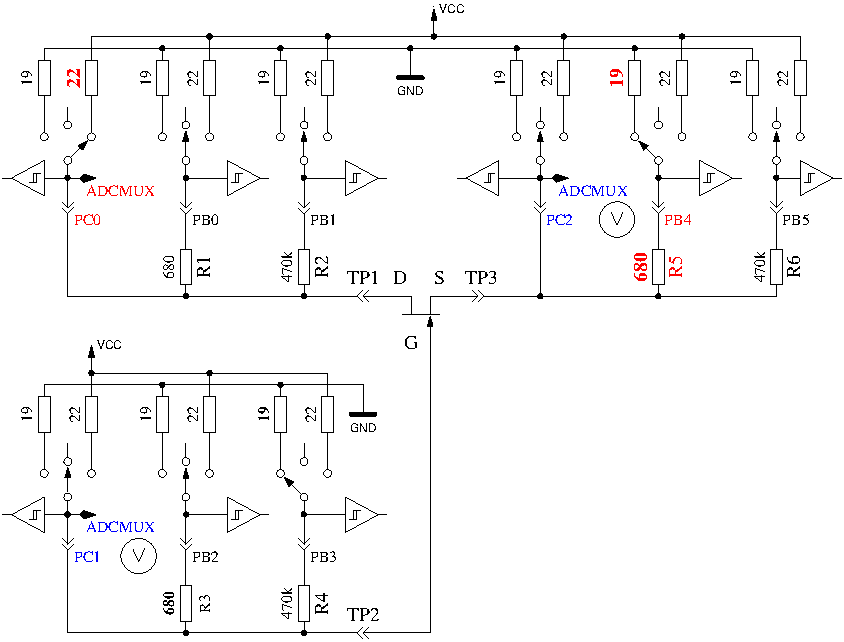
\includegraphics[width=.8\textwidth]{../FIG/JFETcd.pdf}
\caption{Messung von Gate-Source-Spannung und Source-Strom eines N-JFET-Transistors}
\label{fig:JFETcd}
\end{figure}

Wenn das Bauteil keinen Strom zwischen dem positiven Pin und dem negativen Pin ohne ein Signal
auf dem Tristate-Pin hat, sind die nächsten Tests im nächsten Unterkapitel \ref{sec:pnp} beschrieben.
Wenn Strom festgestellt wird, sind die nächsten Tests in dem Dioden-Unterkapitel \ref{sec:diode} beschrieben.

\subsection{Messung eines PNP-Transistors oder eines P-Kanal MOSFETs}
\label{sec:pnp}
Zuerst wird der Stromverstärkungsfaktor in der Kollektor-Schaltung (Emitter-Folger) für den angenommenen
PNP-Transistor gemessen.
Die Messsituation wird in Abbildung \ref{fig:pnpcc} gezeigt.
Wenn die gemessene Basis-Spannung (\(UB\)) über \(9mV\) mit dem \(680\Omega\) Widerstand liegt,
wird die Stromverstärkung hFE berechnet mit \(hFE = \frac{UE-UB}{UB}\). 
Die Spannung \(UE\) ist die Differenz der Emitter-Spannung zu VCC.
Die Differenz des \(22\Omega\) und \(19\Omega\)-Widerstandes wird nicht berücksichtigt.
Wenn die Spannung \(UB\) unter \(10mV\) liegt, wird die Messung mit dem \(470k\Omega\)-Widerstand an der Basis gemacht.
Für diesen Fall wird der Stromverstärkungsfaktor mit \(hFE = \frac{UE \cdot 470000}{UB \cdot (680+22)}\) gebildet.

\begin{figure}[H]
\centering
 \begin{overpic}[width=1.\textwidth]{../FIG/PNPcc.pdf}
  \color{black}
  \put(55,20){\makebox(0,0)[lb]{\footnotesize {Wenn Spannung an PC1 \textless~10mV ist,}}}
  \put(55,17){\makebox(0,0)[lb]{\footnotesize {wird der \textcolor{green}{grün} gezeichnete Zustand benutzt!}}}
 \end{overpic}
\caption{hFE-Messung eines PNP-Transistors in Kollektor-Schaltung}
\label{fig:pnpcc}
\end{figure}

Als Nächstes werden die Tests in Emitter-Schaltung für den angenommenen PNP-Transistor gemacht.
Die positive Seite wird jetzt direkt mit VCC verbunden, der \(680\Omega\)-Widerstand der negativen Seite wird 
mit GND verbunden, wie es in Abbildung \ref{fig:pnpce} gezeigt wird. 
Wenn die negative Seite des Bauteils eine Spannung über \(3,4V\) hat, wenn der \(680\Omega\)-Widerstand auf der Basis-Seite mit
GND verbunden ist, muss es ein PNP-Transistor oder ein P-Kanal-FET sein.
Das kann einfach unterschieden werden durch Prüfen der Basis-Spannung: Wenn sie grösser als \(0,97V\) ist, muss es ein PNP sein.
Für die Messung des Stromverstärkungsfaktors wird anstelle des \(680\Omega\)-Widerstandes der
 \(470k\Omega\)-Widerstand als Basis-Widerstand genommen.
Der Stromverstärkungsfaktor wird berechnet mit \(hFE = \frac{(UC-UC0) \cdot 470000}{UB \cdot (680+19)}\) .
Die Spannung UC0 ist die Spannung am Kollektorwiderstand ohne Basisstrom.
Der höhere Stromverstärkungsfaktor wird als der richtige angenommen, dieser hier oder der
mit der Kollektor-Schaltung bestimmte.


Die Werte, die für den PNP-Transistor herausgefunden wurden, sind nur gültig, wenn ein zweiter Satz
von Messungen gemacht wurde.
Um zu verhindern, dass der PNP-Transistor in der inversen Schaltung (Kollektor und Emitter vertauscht) erkannt
wird, wird dann die Messung mit dem höheren Stromverstärkungsfaktor als richtige Messung genommen.
Wenn die Basis-Spannung kleiner als \(0,97V\) ist, muss es ein P-E-MOS sein.
In diesem Fall wird die Gate-Schwellwertspannung dadurch bestimmt, dass die Spannung am Gate langsam mit dem
 \(470k\Omega\)-Widerstand rauf und runter gezogen wird, bis die Drain-Seite schaltet und dann
die Spannung am Gate gemessen wird.

\begin{figure}[H]
\centering
 \begin{overpic}[width=1.\textwidth]{../FIG/PNPce.pdf}
  \color{black}
  \put(55,21){\makebox(0,0)[lb]{\footnotesize {Schwarzer Zustand wird benutzt beim Test!}}}
  \put(55,17){\makebox(0,0)[lb]{\footnotesize {\textcolor{green}{Grüner} Zustand wird für den}}}
  \put(55,13){\makebox(0,0)[lb]{\footnotesize {Stromverstärkungsfaktor hFE benutzt.}}}
 \end{overpic}
\caption{Prüfung und hFE-Messung eines PNP-Transistors in der Emitter-Schaltung}
\label{fig:pnpce}
\end{figure}

\subsection{Messung eines NPN-Transistors oder eines N-Kanal-MOSFET}
Die Messung eines NPN-Transistors beginnt auf gleiche Weise wie die PNP-Transistor-Messung, nämlich
mit der Messung des Stromverstärkungsfaktors in der Kollektor-Schaltung.
Zuerst wird die Messung mit einem nach VCC geschalteten \(680\Omega\)-Basiswiderstand gemacht.
Wenn die Spannung am Basis-Widerstand zu klein ist, wird stattdessen der \(470k\Omega\)-Widerstand genommen.
Die Messungen werden dann in der Emitter-Schaltung fortgeführt, wie in Abbildung \ref{fig:npnce} gezeigt.
\begin{figure}[H]
\centering
 \begin{overpic}[width=1.\textwidth]{../FIG/NPNce.pdf}
  \color{black}
  \put(55,23){\makebox(0,0)[lb]{\footnotesize {Schwarzer Zustand wird benutzt beim Test!}}}
  \put(55,19){\makebox(0,0)[lb]{\footnotesize {\textcolor{green}{Grüner} Zustand wird für den}}}
  \put(55,15){\makebox(0,0)[lb]{\footnotesize {Stromverstärkungsfaktor hFE benutzt.}}}
 \end{overpic}
\caption{Prüfung und hFE-Messung eines NPN-Transistors in Emitter-Schaltung}
\label{fig:npnce}
\end{figure}
Wenn die Spannung auf der Kollektor Seite unter \(1,6V\) liegt, während der \(680\Omega\)-Basiswiderstand mit
VCC verbunden ist, muss es ein NPN, ein N-Kanal MOSFET oder ein Thyristor (TRIAC) sein.
Mit zwei einfachen Tests kann ein Thyristor oder TRIAC erkannt werden.
Wenn der Gate-Pin für \(10ms\) mit GND verbunden wird und dann stromlos geschaltet wird, sollte
der Strom an der Anode bleiben.
Wenn jetzt der Anoden-Widerstand kurz auf GND geschaltet und dann auf VCC zurückgeschaltet wird,
sollte der Thyristor nicht erneut zünden (stromlos bleiben).
Beachten Sie, dass nur Kleinleistungs-Thyristoren getestet werden können, weil der Haltestrom des
Testers nur \(6mA\) erreichen kann.
Wenn beide Tests einen Thyristor bestätigen, werden weitere Tests in umgekehrter Polarität gemacht,
um ein TRIAC auszuschliessen oder zu bestätigen.

Wenn weder Thyristor noch TRIAC bestätigt wurden, kann es ein NPN oder ein N-Kanal E-MOSFET sein.
Die Basis-Spannung von einem NPN-Transistor wird nahe bei der Emitter-Spannung liegen, so dass dieser Typ sicher
erkannt werden kann.
Der Stromverstärkungsfaktor in der Emitter-Schaltung wird durch 
\(hFE = \frac{(VCC-UC-UC0)\cdot 470000}{(VCC-UB)\cdot (680+22)}\) gebildet.
Wenn die Spannung an der Basis zeigt, dass kein oder wenig Strom fließt, wird das Bauteil ein N-Kanal E-MOS
(Anreicherungs-MOSFET) sein.
In diesem Fall wird die Schwellspannung gemessen, indem die Spannung des Gates langsam mit
dem \(470k\Omega\)-Widerstand nach VCC und GND gezogen wird, darauf wartend, dass das digitale
Eingangs-Signal auf der Drain-Seite schaltet, wobei dann die Gate-Spannung gelesen wird.
Die Messung wird elf Mal wiederholt wie in Abbildung~\ref{fig:eleven} gezeigt und die Ergebnisse addiert.
Diese Summe wird mit Vier multipliziert und durch Neun geteilt, um eine Auflösung in mV zu erhalten.
\begin{figure}[H]
\centering
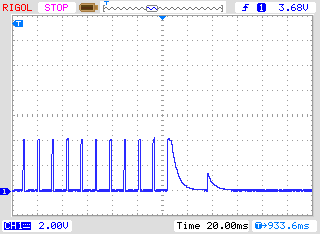
\includegraphics[width=.8\textwidth]{../PNG/IRFU120gate.png}
\caption{Messung der Schwellspannung eines N-Kanal-MOSFET}
\label{fig:eleven}
\end{figure}

\subsection{Vereinfachter Ablauf der Transistorerkennung}

\begin{figure}[H]
\centering
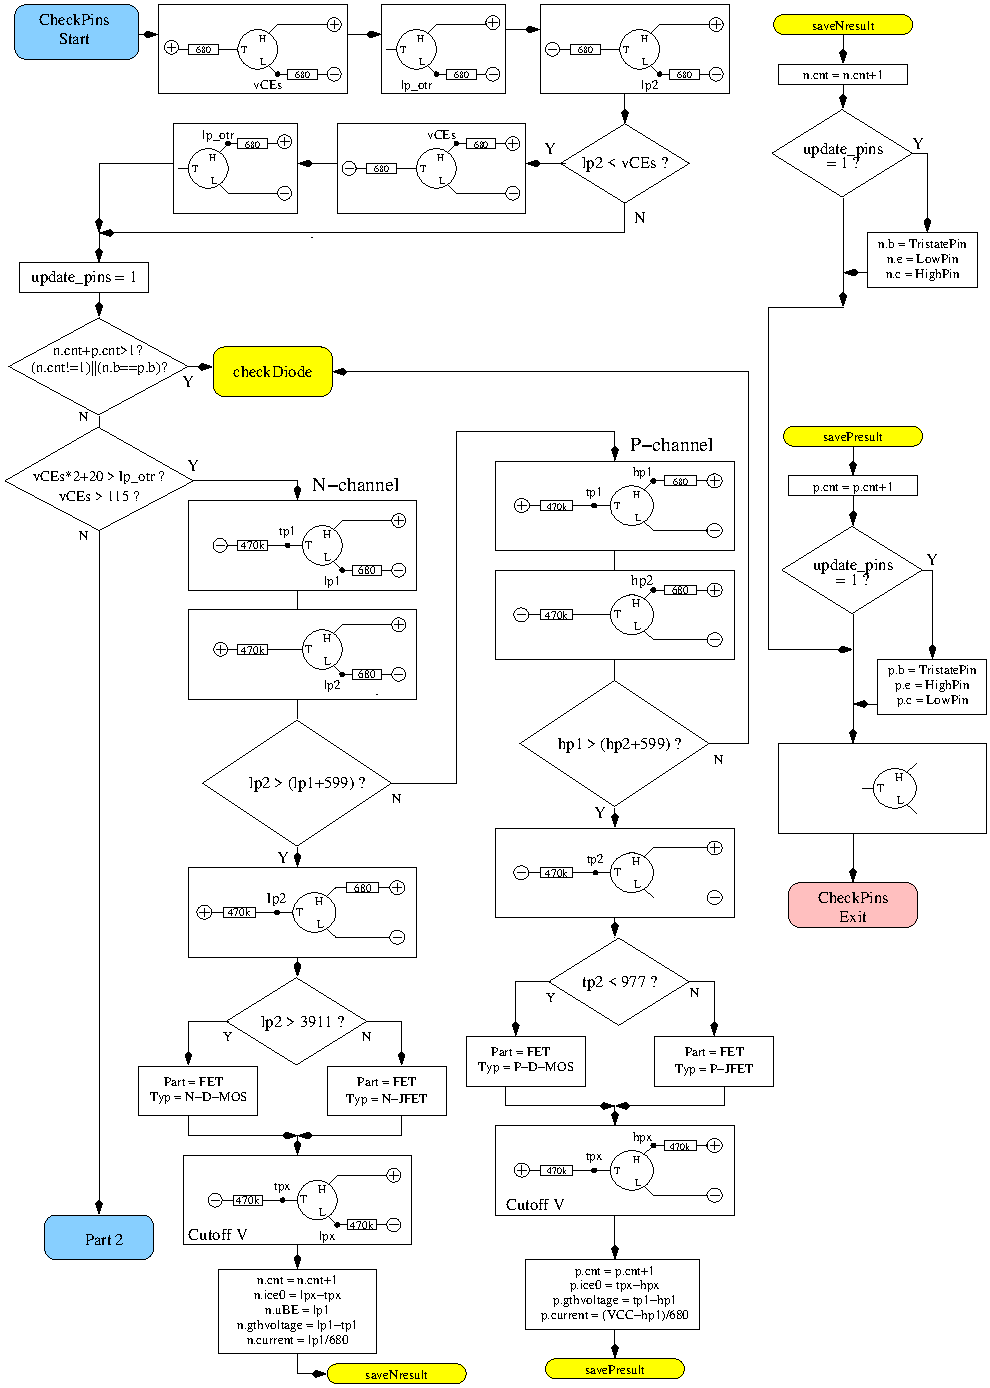
\includegraphics[width=.95\textwidth]{../FIG/CheckSemi1.pdf}
\caption{Ablaufplan der Transistorprüfung Teil 1, JFET und D-MOS}
\label{fig:ChkSemi1}
\end{figure}

\begin{figure}[H]
\centering
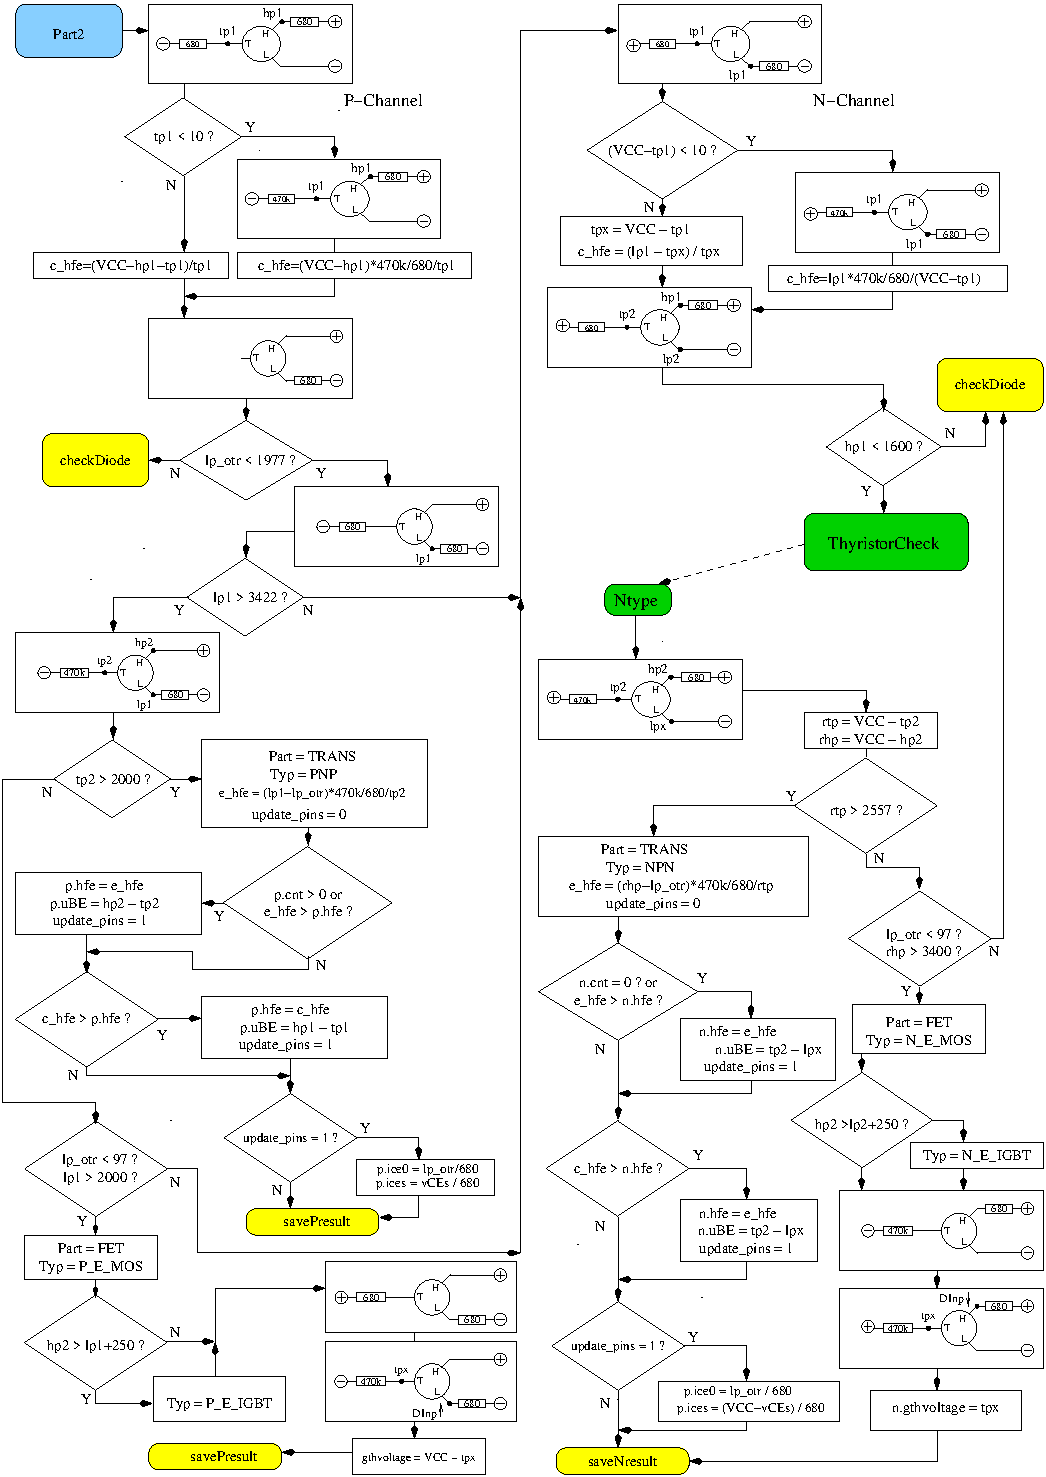
\includegraphics[width=.95\textwidth]{../FIG/CheckSemi2.pdf}
\caption{Ablaufplan der Transistorprüfung Teil 2, BJT und E-MOS}
\label{fig:ChkSemi2}
\end{figure}

\begin{figure}[H]
\centering
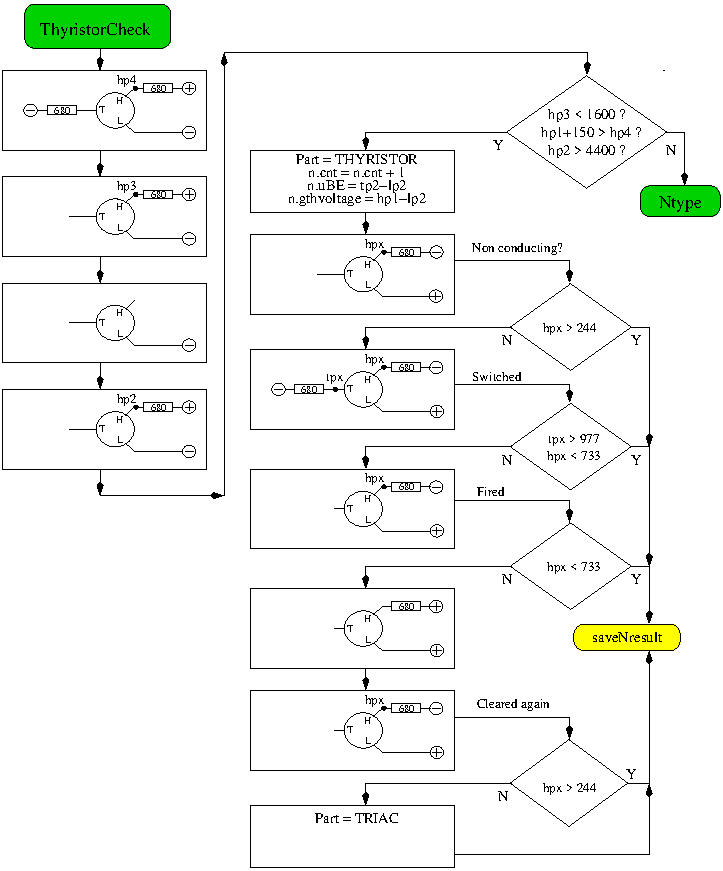
\includegraphics[width=.95\textwidth]{../FIG/CheckSemi3.pdf}
\caption{Ablaufplan der Transistorprüfung Teil 3, Thyristor und Triac}
\label{fig:ChkSemi3}
\end{figure}

\subsection{Messung von Dioden}
\label{sec:diode}
Wenn Strom bei den Vortests festgestellt wurde, wird das Bauteil auf Diodenverhalten geprüft.
Die Flussspannung mit dem \(680\Omega\)-Widerstand muss zwischen \(0,15V\) und \(4,64V\) liegen.
Die Flussspannung mit dem \(680\Omega\)-Widerstand muss grösser als 1,125 Mal der Flussspannung mit dem
 \(470k\Omega\)-Widerstand sein und sechzehn Mal die Flussspannung mit dem \(470k\Omega\)-Widerstand muss
grösser als die Flussspannung mit dem \(680\Omega\)-Widerstand sein.
Zusätzlich darf die anschließende nochmalige Messung mit dem \(470k\Omega\)-Widerstand keine höhere Spannung als die
Messung mit dem \(680\Omega\)-Widerstand ergeben.
Ich hoffe, dass ein Bauteil mit diesem Verhalten immer eine Diode ist.
Die Erkennung des Diodenverhaltens durch den fehlenden Stromfluß in der Gegenrichtung ist nicht
möglich bei antiparallelen Dioden.
Bei einer Einzeldiode wird zusätzlich der Sperrstrom der Diode bei \(5V\) mit dem \(470k\Omega\) Widerstand
gemessen. Die Auflösung beträgt etwa \(2nA\).
Bei größeren Restströmen als \(5,3\mu A\) (Spannung am Widerstand größer als \(2,5V\)) wird
 mit dem \(680\Omega\) Widerstand gemessen.
Dann beträgt die Auflösung nur etwa \(1\mu A\).
Außerdem wird bei Einzeldioden eine Kapazitätsmessung in Sperr-Richtung durchgeführt. 

\subsection{Ergebnisse der verschiedenen Messungen}
Die folgenden drei Tabelle zeigen die Ergebnisse verschiedener Bauteile 
eines ATmega8-, ATmega168- und ATmega328-Prozessors.
Die Messung der Sperrschichtkapazität für die Doppeldiode MBR4045PT gelingt
nur gekühlt. Die Ursache hierfür ist der hohe Reststrom der \(40A\)-Diode. Ebenso kann für die Basis-Emitter-Strecke 
des Germanium-Transistors AC128 die Sperrschichtkapazität nur im
gekühlten Zustand gemessen werden. 

\begin{table}[H]
  \begin{center}
    \begin{tabular}{| l | c | c | c | c |}
    \hline
           & Mega8@8MHz          & Mega168 @8MHz       & Mega328 @8MHz     \\
 Diode Typ &                     &                     &                   \\
    \hline
    \hline
1N4148     & Diode, 715mV,        & Diode, 718mV,            & Diode, 715mV,           \\
           &               1pF    &               0pF, 2nA   &               1pF, 4nA  \\
    \hline
1N4150     & Diode, 665mV,        & Diode, 672mV,            & Diode, 666V,           \\
           &               1pF    &               1pF, 4nA   &              2pF, 6nA  \\
    \hline
BA157      & Diode, 619mV,        & Diode, 621V,              & Diode, 615mV,            \\
           &               19pF   &              17pF, 12nA   &               18pF, 12nA \\
    \hline
BY398      & Diode, 538mV,        & Diode, 541mV,             & Diode, 537mV,            \\
           &               16pF   &               14pF, 63nA  &               15pF, 63nA \\
    \hline
1N4007     & Diode, 650mV,        & Diode, 655mV,            & Diode, 650mV,           \\
           &               13pF   &               10pF, 6nA  &               13pF, 6nA \\
    \hline
LED green  & Diode, 1.96V, 5pF    & Diode, 1.95V, 4pF   & Diode, 1.95V, 4pF \\
    \hline
ZPD2,7     & 2xDi, 743mV, 2.53V   & 2xDi, 737mV, 2.52V  & 2xDi, 733mV, 2.51V \\
    \hline
BU508A B+E & Diode, 609mV,        & Diode, 611mV,                & Diode, 606mV,              \\
           &               5.15nF &               5.20nF, 0.39uA &               5.25nF, 0.4uA\\
    \hline
BU508A B+C & Diode, 582mV,        & Diode, 586mV,             & Diode, 587mV,            \\
           &               256pF  &               255pF, 21nA &               259pF, 19nA\\
    \hline
AC128 B+E  & Diode, 272mV,        & Diode, 277mV,              & Diode, 273mV,             \\
           &               0pF    &               0pF, 2.2uA   &               0pF, 2.3uA  \\
    \hline
AC128 B+E  &                      &                     & Diode, 349mV,               \\
gekühlt    &                      &                     &               140pF, 0.57uA \\
    \hline
MBR20100CT & 2xDi, 337mV, 337mV   & 2xDi, 338mV, 338mV  & 2xDi, 336mV, 335mV  \\
    \hline
MBR20100CT & Diode, 337mV,        & Diode, 339mV,             & Diode, 337mV,            \\
           &               345pF  &               351pF, 29nA &               350pF, 25nA\\
    \hline
MBR4045PT  & Diode, 243mV,        & Diode, 233mV,               & Diode, 235mV,              \\
gekühlt    &               1.80nF &               1.94nF, 1.7uA &               1.95nF, 1.8uA\\
    \hline
SK14       & Diode,    mV,        & Diode,    mV,               & Diode, 263mV,              \\
           &                  0pF &                   pF,    nA &               0pF, 0.57uA\\
    \hline
SK14       & Diode,    mV,        & Diode,    mV,               & Diode, 334mV,              \\
gekühlt    &                   nF &                   pF,    nA &               88pF, 4nA\\
    \hline
SF38G      & Diode, 519mV,        & Diode, 521mV,            & Diode, 516mV,            \\
           &               107pF  &               105pF, 2nA &               106pF, 2nA \\
    \hline
    \end{tabular}
  \end{center}
  \caption{Messergebnisse der Dioden-Tests}
  \label{tab:diodes} 
\end{table}

\begin{table}[H]
  \begin{center}
    \begin{tabular}{| l | c | c | c | c | c |}
    \hline
 Transistor & Typ & Mega8           & Mega328        & Mega328         & Mega328 \\
    Typ     &     & common-         & maximum        & common-         & common- \\
            &     & collector       &                & collector       & emitter \\
    \hline
    \hline
BU508A      & NPN & B=9, 601mV      &  B=9, 597mV    &   B=9, 598mV    & B=4, 484mV \\
    \hline
2N3055      & NPN & B=20, 557mV     &  B=21, 550mV   &   B=21, 550mV   & B=6, 442mV \\
    \hline
BC639       & NPN & B=148, 636mV    &  B=172, 629mV  &   B=172, 629mV  & B=158, 605mV \\
    \hline
BC640       & PNP & B=226, 650mV    &  B=176, 609mV  &   B=171, 655mV  & B=177, 608mV \\
    \hline
BC517       & NPN & B=23.9k, 1.23V  &  B=24.8k, 1.22V&   B=25.1k, 1.22V & B=764, 1.23V \\
    \hline
BC516       & PNP & B=75.9k, 1.21V  &  B=76.2k, 1.20V&   B=76.2k, 1.20V & B=760, 1.23V \\
    \hline
BC546B      & NPN & B=285, 694mV    &  B=427, 687mV  &   B=427, 687mV   & B=369, 683mV \\
    \hline
BC556B      & PNP & B=304, 704mV    &  B=254, 668mV  &   B=235, 709mV   & B=255, 668mV \\
    \hline
AC128 (Ge.) & PNP & B=63, 191mV     &  B=59, 191mV   &   B=57, 193mV    & B=43, 117mV \\
    \hline
BUL38D      & NPNp & B= 37, 627mV    &  B=41, 617mV  &   B=40, 624mV    & B=36, 562mV \\
parasitär   & PNPn & B= 11, 654mV    &  B=81, 543mV  &   B=10, 656mV    & B=83, 541mV \\
    \hline
BRY55/200   & Thyrist. &  0.84V      &  0.81V        &  0.82V           &  0.82V \\
    \hline
MAC97A6     & Triac &   0.92V        &  0.90V        &  0.91V           &  0.90V    \\
    \hline
    \end{tabular}
  \end{center}
  \caption{Messergebnisse der Tests mit bipolaren Transistoren}
  \label{tab:bipolar} 
\end{table}

Die Ergebnisse der Transistormessungen unterscheiden sich teilweise erheblich von den Werten der Version 
von Markus Frejek. Zum Beispiel wird für den Darlington-Transistor BC517 von
der früheren Software ein hFE von nur 797 statt 77200 gemessen. 
Dies hängt damit zusammen, dass die Stromverstärkung bei der neuen Version auch mit der
Kollektorschaltung gemessen wird.
Dies zeigen auch die Ergebnisse der neuen Version in der Emitterschaltung (common emitter),
wie man in der letzten Spalte der Tabelle \ref{tab:bipolar} sehen kann.
Die Basis-Emitter-Spannung wurde früher mit einem separaten Diodentest mit \(1438mV\) ermittelt.
Jetzt wird die angegebene Basis-Emitter-Spannung im Zustand der Verstärkungsmessung (\(1,20V\)) ermittelt.
Der BUL38D-Transistor enthält eine Schutzdiode über der Anode und dem Kollektor des NPN-Transistors,
wodurch ein parasitärer PNP-Transistor mit vertauschtem Basis-Kollektor Anschluss entsteht.
In der Softwareversion 1.10k werden beide Transistoren erkannt und durch das angehängte p auf
den weiteren Transistor hingewiesen.
Der richtige Transistor (NPN) wird durch einen Vergleich der Sperrschichtkapazitäten herausgefunden.
Es wird angenommen, dass der mit der höheren Sperrschichtkapazität der richtige Transistor ist.
Wenn während der Ergebnisanzeige die Start-Taste gedrückt ist, werden die Parameter des parasitären Transistors
angezeigt. Dabei wird wieder mit PNPn auf die andere Transistorstruktur hingewiesen.
Die weitere Transistorstruktur entsteht nur bei der Integration der Schutzdiode in unmittelbarer
Nachbarschaft des Transistors in das gleiche Halbleitermaterial, nicht bei einer externen Diode.

In der folgenden Tabelle \ref{tab:germanium} werden die Messergebnisse von Germanium-Transistoren gezeigt, die wegen den
stark temperaturabhängigen Kollektor-Restströmen besonders problematisch sind.
Es werden die Ergebnisse der Urversion von Markus F. und die Ergebnisse der 1.10k Version
miteinander verglichen. Die 1.10k Version mißt die Stromverstärkung sowohl in der
Kollektorschaltung als auch in der Emitterschaltung mit Berücksichtigung des Kollektor-Ruhestroms,
 wobei die höhere Stromverstärkung ausgegeben wird.
Der Kollektor-Ruhestrom wurde in älteren Versionen nicht berücksichtigt.

\begin{table}[H]
  \begin{center}
    \begin{tabular}{| l | c | c | c |}
    \hline
 Transistor & Mega8 @1MHz          & Mega168 @8MHz       & Mega328 @8MHz    \\
    Typ     & Ur-Version          & Version 1.10k       & Version 1.10k  \\
            & Markus F.           &                     &        \\
    \hline
    \hline
AC128       & PNP, B=52, 279mV    & PNP, B=59, 184mV    & PNP, B=59, 191mV    \\
    \hline
AC116-65    & PNP, B=505, 378mV   & PNP, B=72, 146mV    & PNP, B=72, 149mV    \\
    \hline
AC116-145   & PNP, B=485, 294mV   & PNP, B=146, 161mV    & PNP, B=146, 163mV   \\
    \hline
AC176-65    & NPN, B=98, 235mV    & NPN, B=58, 94mV    & NPN, B=56, 96mV     \\
    \hline
GC122       & PNP, B=84, 368mV    & PNP, B=55, 117mV    & PNP, B=56, 117mV    \\
    \hline
GC301       & PNP, B=48, 289mV    & PNP, B=39, 184mV    & PNP, B=39, 188mV    \\
    \hline
AD161       & NPN, B=360, 230mV   & NPN, B=296, 126mV   & NPN, B=298, 128mV    \\
    \hline
AD162       & PNP, B=2127, 280mV  & PNP, B=89, 107mV    & PNP, B=89, 107mV    \\
    \hline
    \end{tabular}
  \end{center}
  \caption{Messergebnisse der Tests mit bipolaren Germanium-Transistoren}
  \label{tab:germanium} 
\end{table}

In der Tabelle \ref{tab:mos} werden die Ergebnisse einiger Feldeffekttransistoren-Messungen gezeigt.
Ein gemessenen Parameter der E-MOS-Typen ist Gate-Source-Schaltspannung,
bei der das digitale Eingangssignal des ATmega eines am \(680\Omega\) Drain-Widerstand 
angeschlossenen Signals schaltet.
Bei sehr schneller Änderung der Gatespannung wegen einer kleinen Gatekapazität 
ist die ermittelte Spannung etwas ungenau.
Beim BS250 ändert sich die Gatespannung von \(2,6V\) auf \(2,5V\), wenn man einen zusätzlichen
\(10nF\) Kondensator an Gate-Source anschließt.

Ein anderer gemessener  Parameter ist die Gatekapazität.
Die Gatekapazität wird ermittelt indem sowohl Source als auch Drain auf GND Potential gelegt wird.
Bei IGBTs reicht oft die Gatespannung von \(5V\) des Testers nicht zur Ansteuerung aus.
Meistens wird dann nur die Emitter-Kollektor Schutzdiode erkannt. 
In diesem Fall kann eine an den Gatepin angeschlossene Batterie mit etwa \(3V\) reichen,
um die Erkennung zu ermöglichen. Der andere Pol der Batterie wird dann anstelle des Gatepins
an den Testpin (TP) des Testers angeschlossen.
Bei richtiger Polarität der Batterie wird dann die Erkennung des IGBTs ermöglicht.
Die angezeigte Gate-Emitter Schaltspannung muß dann um die Batteriespannung erhöht werden,
um die wahre Schaltspannung zu erhalten.

Bei JFET-Transistoren wird in den Datenblättern oft der Idss-Kennstrom genannt,
der Strom im Drain bei einer Gate-Source-Spannung von 0V.
Hier wird aber der Strom angegeben, der sich durch einen \(680\Omega\) Lastwiderstand auf der
Source-Seite des JFET ergibt.
Der Lastwiderstand erzeugt für das Gate eine Gegenspannung Vgs,
die ebenfalls angegeben wird.
Mit einem \(470k\Omega\) Lastwiderstand auf der Source-Seite des JFET ist der Source-Drain Strom
fast 0. Damit läßt sich die Gate-Source Cutoff Spannung Vgs\_off hinreichend genau bestimmen,
sofern sie unter \(5V\) liegt.
Mit diesen beiden Arbeitspunkten läßt sich aufgrund der quadratischen Strom-Kennlinie ein Igss
schätzen. Sofern der geschätzte Strom unter \(40mA\) liegt, wird noch eine zusätzliche Messung
ohne Widerstand am Source Anschluß gemacht. 
Über die Spannung am Source-Anschluß kann ein weiterer Stromwert bestimmt werden. 
Mit diesem höheren Stromwert und der Gate-Source Spannung wird der Strom Idss noch einmal mit
der quadratischen Strom-Kennlinie berechnet, sofern ein Wert von \(40mA\) nicht überschritten wird.
Wegen des symmetrischen Aufbaus der JFETs kann Drain und Source nicht unterschieden werden.

\begin{table}[H]
  \begin{center}
    \begin{tabular}{| l | l | c | c | c |}
    \hline
             &         & Mega8 @8MHz       & Mega168 @8MHz    & Mega328 @8MHz \\
 Transistor  & Typ     &                  &                  &               \\
    \hline
    \hline
ZVNL120A     & N-E-MOS & D, 1.6V, 147pF   & D, 1.5V,141pF    & D, 1.5V, 140pF \\
    \hline
IRF530N      & N-E-MOS & D, 3.6V, 1.55nF  & D, 3.6V, 1.54nF  & D, 3.6V, 1.54nF \\
    \hline
BS170        & N-E-MOS & D, 2.6V, 78pF    & D, 2.6V, 68pF    & D, 2.6V, 68pF \\
    \hline
IRL3803      & N-E-MOS & D, 2.3V, 9.81nF  & D, 2.3V, 9.71nF  & D, 2.3V, 9.74nF \\
    \hline
IRFU120N     & N-E-MOS & D, 4.2V, 909pF   & D, 4.2V, 913pF   & D, 4.2V, 911pF \\
    \hline
BUZ71A       & N-E-MOS & D, 3.2V, 714pF   & D, 3.2V, 708pF   & D, 3.2V, 705pF \\
    \hline
ZVP2106A     & P-E-MOS & D, 3.2V, 122pF   & D, 3.2V,115pF    & D, 3.2V, 116pF \\
    \hline
IRF5305      & P-E-MOS & D, 3.6V, 2.22nF  & D, 3.6V, 2.22nF  & D, 3.6V, 2.22nF \\
    \hline
BS250        & P-E-MOS & D, 2.6V, 53pF    & D, 2.6V, 43pF    & D, 2.6V, 44pF \\
    \hline
IRFU9024     & P-E-MOS & D, 3.5V, 937pF   & D, 3.6V, 945pF   & D, 3.5V, 933pF \\
    \hline
J310         & N-JFET  & 3.1mA Vgs=2.2V   & 3.1mA Vgs=2.2V   & 3.1mA Vgs=2.2V \\
Idss=24-60mA &         &                  &                  & Idss=35mA      \\
    \hline
2N5459       & N-JFET  & 2.1mA Vgs=1.5V   & 2.1mA Vgs=1.5V   & 2.1mA Vgs=1.5V \\
Idss=4-16mA &          &                  &                  & Idss=8.2mA     \\
    \hline
BF256C       & N-JFET  & 3.4mA Vgs=2.4V   & 3.4mA Vgs=2.4V   & 3.4mA Vgs=2.4V \\
Idss=11-18mA &         &                  &                  & Idss=14mA      \\
    \hline
BF245A       & N-JFET  & 1.1mA Vgs=.75V   & 1.1mA Vgs=0.75V  & 1.1mA Vgs=0.75V \\
Idss=2-6mA   &         &                  &                  & Idss=3.6mA      \\
    \hline
BF245B       & N-JFET  & 2.5mA Vgs=1.7V   & 2.5mA Vgs=1.7V   & 2.5mA Vgs=1.7V \\
Idss=6-15mA  &         &                  &                  & Idss=10mA      \\
    \hline
BF245C       & N-JFET  & 3.9mA Vgs=2.7V   & 3.9mA Vgs=2.7V   & 3.9mA Vgs=2.7V \\
Idss=12-25mA &         &                  &                  & Idss=17mA    \\
    \hline
J175        & P-JFET   & 3.2mA Vgs=2.2V   & 3.2mA Vgs=2.2V   & 3.2mA Vgs=2.2V \\
Idss=7-60mA &          &                  &                  & Idss=26mA      \\
    \hline
2N5460      & P-JFET   & 0.78mA Vgs=0.54V & 0.77mA Vgs=0.54V & 0.78mA Vgs=0.54V \\
Idss=1-5mA  &          &                  &                  & Idss=2.6mA       \\
    \hline
BSS139      & N-D-MOS  & 1.7mA Vgs=1.2V  & D, 1.7mA Vgs=1.2V & D, 1.7mA Vgs=1.2V \\
    \hline
BSS169      & N-D-MOS  & 2.6mA Vgs=1.8V  & D, 2.6mA Vgs=1.8V & D, 2.6mA Vgs=1.8V \\
    \hline
GP07N120    & N-E-IGBT & C=3.81nF Vt=4.2V & C=3.76nF Vt=4.2V & C=3.74nF Vt=4.2V \\
    \hline
IRG4PC30    & N-E-IGBT &                  &                  & C=2.22nF         \\
mit Bat.    &          &                  &                  & Vt=2.0V+3.2V \\
    \hline
    \end{tabular}
  \end{center}
  \caption{Messergebnisse der FET-Tests}
  \label{tab:mos} 
\end{table}
